%-------------------------------------------------------------------------------
\chapter{Neurális hálózatok és a Deep Learning}\label{chap:neuralis-halozatok-es-a-deep-learning}
%-------------------------------------------------------------------------------
%Ebben a fejezetben szeretném összegezni megszerzett tudásomat a neurális hálózatokról és a Deep Learning-ről, magyarul mély tanulásról. 

\section{A neurális hálózatok elmélete}
\label{sect:neuralNetworkTheory}
Olyan számítási modellel, amelynek alapját az idegrendszer hálózata adja először  Warren McCulloch és Walter Pitts 1943-ban foglalkozott az ,,A Logical Calculus of the Ideas Immanent in Nervous Activity'' című publikációjukban. Később Donald Hebb tanulással kapcsolatos megfigyeléseivel elindultak a mesterséges neurális hálókkal kapcsolatos kísérletezések.\cite{neural2006}\cite{nielsen2015}
Kiderült, hogy ezek a struktúrák kiválóan alkalmasak osztályozási és regresszió számítási problémák megoldására, és a mai gépi tanulással kapcsolatos fejlesztések középpontjába került.

A mesterséges neurális hálózatok egy viszonylag egyszerű modellen alapulnak. Minden neuron a hozzá kapcsolódó neuronok ingereinek összessége alapján ingerli a többi neuront melyekhez ő kapcsolódik, ekképpen az ingerület egy irányba halad a kapcsolatok mentén. Hogy a hálózat áttekinthető legyen, rendezzük a neuronokat rétegekbe úgy, hogy egy réteg neuronjai az ingerületet a közvetlen felső réteg neuronjaitól kapja, és a válasz ingert a közvetlenül alatta lévő réteg neuronjainak továbbítja.

\begin{figure}[h]
	\centering
%	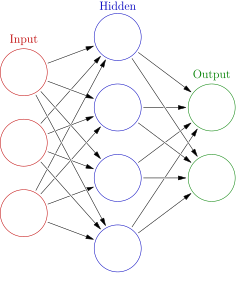
\includegraphics[width=0.9\textwidth]{Colored_neural_network.svg}
	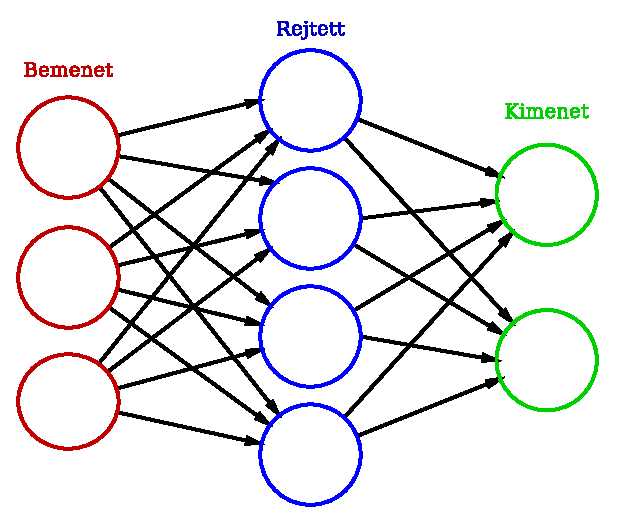
\includegraphics[width=0.3\columnwidth]{fig/neural_network}
	\caption{neurális hálózat réteges szerkezete \footnotesize forrás: en.wikipedia.org/wiki/Artificial\_neural\_network}
	\label{fig:neuralNet}
\end{figure}

A \ref{fig:neuralNet} ábrán a csúcsok jelentik a neuronokat és az élek a szinapszisok, melyeken az ingerület vándorol. Egy hálózat 3 nagyobb részre tagolódik:
\begin{enumerate*}[label={\alph*)},font=\bfseries]
	\item bemeneti réteg
	\item rejtett rétegek
	\item kimeneti réteg.
\end{enumerate*}
A bemeneti réteg csúcsai legtöbbször az adatot reprezentáló konstansok jelentik, tehát az egy egyszerű vektor.
Egy neuronban két művelet történik: a bementek összegzése és egy aktiváló függvény kiértékelés. Az összegzést a felsőbb rétegből érkező jelekre elvégezzük:
\begin{displaymath}
	s = \sum_i{w_ix_i}+b = \vec{w}\cdot\vec{x} + b
\end{displaymath}
ahol $x_i$ a felső réteg i.-ik neuronjának kimenete, $w_i$ az i.-ik neuron szinapszisához tartozó súly, mellyel a szinapszis "erősségét" határozzuk meg. Az "s" összeghez hozzáadunk még egy $b$  büntetőtagot, ami neuron aktiválási küszöbe lesz.
Az aktivációs függvény adja a neurális hálózat kimenetét, melynek paramétere $s$.
A neurális hálózatok fejlesztésekor sokféle függvényt találtak alkalmasnak aktivációs függvény gyanánt. Közös jellemzőjük, hogy inflexiós pontjuk $x=0$ helyen van, illetve 0-ban nem deriválható függvények esetén a töréspont esik ide.

A szemléletesség kedvéért tekintsünk meg az egyrétegű perceptront, vagyis egy egyetlen rétegből álló neurális hálózatot $k$ darab neuronnal. A bemenet legyen az $\vec{x}=(x_1,\dots,x_n)$ vektor. A szinapszisok súlyait a $W=\{w_{ij}:i=1\dots n,j=1\dots k\}$  mátrix ($\vec{w}_i$ az i. bemeneti adatból kiinduló szinapszisokhoz tartozó súlyok vektora lesz), a neuronok  büntetőtagját a $\vec{b}=(b_1,\dots,b_k)$ tartalmazza. Az aktivációs függvény $f$. A hálózat kimenetét, vagyis a  $\vec{y}=(y_1,\dots,y_k)$ elemeit megkapjuk a következőképpen:
\begin{displaymath}
	y_j = f(\vec{w}_i\cdot\vec{x}+b_j)
\end{displaymath}

A fentiekből látszik, hogy a hálózat tervezésénél annak négy tulajdonságát kell meghatároznunk:
\begin{enumerate*}
	\item a rétegek és azok neuronjainak számát
	\item a neuronok aktivációs függvényét (rétegenként egy típusú függvény az összes neuronra)
	\item a szinapszisok súlyát ($W=(\vec{w_1},\cdots\vec{W_n})$)
	\item a neuronok aktiválási küszöbét ($\vec{b}$).
\end{enumerate*}
Minden réteghez külön $W$ mátrixot és $\vec{b}$ vektort kell meghatározni. \textbf{Az egyszerűség kedvéért néha az egy réteghez tartozó $W$-t és $\vec{b}$-t együttesen nevezik a réteg \emph{súlyainak}}. Ez nagyon sok külön meghatározandó változót jelent, tehát csak az 1. és 2. tulajdonság meghatározása elvárható. Kell egy algoritmus, mellyel az egész hálózathoz tartozó paraméterek sokasága -- vagyis minden réteg súlyának paraméterei -- meghatározható.


\section{Deep Learning}
%A Deep Learning-ről szerzett tudásom javát F. Cholett könyvéből\cite{chollet} szereztem, melynek a témához kapcsolódó részleteit alább bemutatom.
Chollet könyvében részletesen kifejti mit is értünk \emph{Deep Learning} alatt, hogyan kapcsolódik a gépi tanulás fogalmához.\cite{chollet}

A gépi taunlás egy teljesen más programozási paradigmát jelent, ugyanis a klasszikus programozás során a feldolgozandó adatokhoz a programozó adja az adat feldolgozásának szabályait, amit végig követve a gép kiszámítja a kívánt eredményt. Ezzel szemben a gépi tanulás során a programozó az adathoz  a kívánt eredményt adja meg, amiből a gép felállítja a megoldáshoz vezető szabályokat.%\cite{Chollet}

A Deep Learning más néven a mély tanulás a gépi tanulás egy fajtája. Chollet szerint a név arra utal, hogy a kezdeti adaton több transzformációt végrehajtva egymás után egyre közelebb kerülünk egy olyan reprezentációhoz, ami megfelel a kívánalmainknak. Ezzel kontrasztban beszélhetünk sekély tanulásról, amikor kevés, egy vagy két transzformáció után kapjuk meg az adat megfelelő reprezentációját.%\cite{Chollet}
A neurális hálózatok rétegeltsége adja a \emph{mélységet} a gépi tanulásban. Eredeti elgondolás szerint minden egyes neuron-réteg egyre összetettebb tulajdonságokat ismer fel a bemeneti adatból. Valójában a rétegenkénti transzformációk egyre kisebb összetettségű hipotézis térbe visznek át, a reprezentáció egyre kevesebb -- a felhasználó számára fölösleges -- információt tartalmaz. Minél több réteg van a hálózatban, annál \emph{mélyebb} a modell.

\begin{figure}[h]
	\centering
	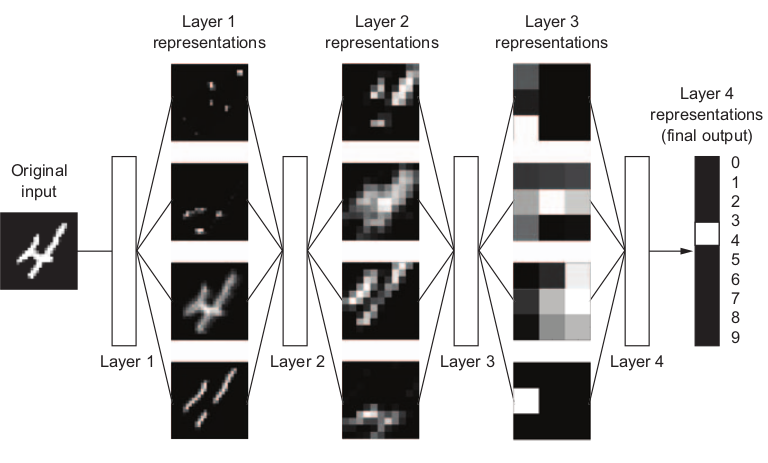
\includegraphics[width=0.8\columnwidth]{fig/digit_classification.png}
	\caption{írott szám hozzárendelése az ábrázolt számértékhez \footnotesize forrás:\cite{chollet}}
	\label{fig:digit_classification}
\end{figure}

Itt kapcsolódik össze a neurális hálózat és a mély tanulás. Az \ref{sect:neuralNetworkTheory} alfejezetben kifejtettem, hogy a neurális hálózat szinapszisainak paraméterezéséért felelős $W$ mátrixok és a neuronok küszöbszintjének állítására szolgáló $\vec{b}$ vektorok összes koordinátájának száma hatalmas lehet, --~alkalmazástól függően több százezer, akár millió, egymástól független változóról beszélünk~-- tehát beállításukhoz valamilyen algoritmusra van szükség. Ezért a neurális hálózatok másik komponense, egy tanulási algoritmus, mely beállítja ezen paramétereket. Négy  megközelítés létezik, amikor gépi tanulásról van szó.

\emph{Ellenőrzött tanulás} során a neurális hálózatnak felcímkézett adatokat adunk meg, tehát olyan $y$ értéket  rendelünk az $x$ mintákhoz, amilyet szeretnénk, hogy a hálózat produkáljon. Ezen $z=(x,y)$ összerendezések halmazát \emph{tanítókészletnek} hívjuk. A hálózat leképezi az adatot a meghatározott reprezentációvá. A tanuló algoritmus ebből és a címkéből egy \emph{veszteség függvény} kiszámításával meghatározza, hogy mekkora az eltérés, a valamilyen értelemben vett távolság a kapott és az elvárt eredmény között. Ez alapján frissíti a $W$ mátrixot és $\vec{b}$ vektorokat.

\emph{Ellenőrizetlen tanulás}, mely során az adatokat nem címkézzük fel, hanem arra vagyunk kíváncsiak, hogy miféle összefüggések állnak fenn közöttük. Ezt a módszert adatbányászat során alkalmazzák. 

Az \emph{Önellenőrzött tanulás} hasonló az ellenőrzötthöz, azonban az adatok felcímkézését nem emberi erővel végezzük, hanem az adatokból állítjuk elő valamilyen heurisztikát felhasználva. Egyik alkalmazási területe az autóenkóderek tanítása.

A \emph{Megerősítéses tanulás} egy újfajta megközelítése a neurális hálózatok alkalmazásának. Ennél a metodikánál a hálózatot egy ágens alkalmazza, így a hálózat bemenete az ágens által megfigyelt környezet a kimenete pedig valamilyen cselekedet, beavatkozás és tanítás során az ágens igyekszik valamilyen környezetbeli értéket maximalizálni. Gyakori alkalmazás valamilyen játékot játszó ágens, ahol azt tanulja, adott helyzetekre milyen reakcióval tudja maximalizálni játékbeli pontszámát.
Vizsgálódásomat az \emph{ellenőrzött tanulásra} korlátoztam, így a továbbiakban ennek tükrében folytatom dolgozatomat.

\section{Függvények, algoritmusok}\label{sec:fuggvenyek-algoritmusok}
Az alábbiakban szeretném megfogalmazni a neurális hálózatokban alkalmazott tipikus függvényeket és algoritmusokat.

\subsection{Neuronok aktivációs függvényei}
Mint korábban kifejtettem minden neuron kimenete egy függvény kiértékelése, melynek paramétere a bemenetek súlyozott összege. Ezt a függvényt hívjuk aktivációs függvénynek. 

\paragraph{A szigmoid függvény}
Az utolsó, kimeneti neuronok rétegének aktivációs függvényeként alkalmazzuk, ahol a várt eredmény egyetlen valószínűségi érték. Ez bináris osztályozási problémák esetén alkalmazandó, tehát a program célja, hogy egy bemeneti adatról eldöntse, hogy az egy bizonyos kategóriába esik-e vagy sem, illetve erről mekkora "magabiztossággal" döntött.
\begin{equation}
	\sigma(x)= \frac{1}{1+e^{-x}}
	\label{eq:sigmoid}
\end{equation}\

\paragraph{A softmax függvény}
A kimeneti réteg aktivációs függvénye. $D$ dimenziójú $x$ vektorok koordinátáit normalizálja, másként fogalmazva egy tetszőleges $D$ elemű szám n-est azon $D$ elemű n-esek halmazába képezi, melyek elemeinek összege 1. Így tehát a $x$ koordinátái egy diszkrét valószínűségi eloszlás értékkészlete.\cite{wiki:softmax}
\begin{equation}
\sigma(x_i)=\frac{e^{x_i}}{\sum_{j=1}^{D}e^{x_i}},\quad i = 1,\dots,D
\label{eq:softmax}
\end{equation}
Éppen ezért többosztályos problémáknál használatos.A hálózat egy mintára adott válasza annak a diszkrét valószínűségi változónak az eloszlása, mely a minta egy adott kategóriába tartozásának a valószínűségét adja meg.

\paragraph{ReLu}
Teljes néven \emph{rectified linear unit} függvény vagy közismerten rámpafüggvény a rejtett neuron rétegek aktivációs értéke szokott lenni. Először 2011-ben mutatták be, hogy hatékonyabban taníthatóak a neurális hálózatok, mintha csak szigmoid függvényt használnánk neuronok aktivációs függvényeként.\cite{wiki:relu}
\begin{equation}
	f(x) = max\{0,x\}
	\label{eq:relu}
\end{equation}

\begin{figure}[h]
	\centering
	\begin{subfigure}[b]{0.3\textwidth}
		\def\svgwidth{0.5\columnwidth}
		\input{fig/Logistic-curve.pdf_tex}
		\caption{Szigmoid függvény}
		\label{fig:sigmoid}
	\end{subfigure}
	~
	\begin{subfigure}[b]{0.3\textwidth}
		\def\svgwidth{0.5\columnwidth}
		\input{fig/Ramp_function.pdf_tex}
		\caption{ReLu függvény}
	\end{subfigure}
	\caption{Aktivációs függvények grafikonja}
\end{figure}

\subsection{Veszteség függvények}
A neurális hálózat tanításához szükséges meghatároznunk egy $c(\vec{y},\vec{y'})$ veszteségfüggvényt, mely megadja a hálózat kimenetének eltérését az elvárt eredményhez képest adott súlyok mellett. Ezt az eltérést egy skalárértékként képezi le. Tanítás során ezt a függvényt kell minimalizálni.
%Formálisan egy $c:W\times B \mapsto \mathbb{R}^+$ függvény, $W,B$, a súlyokat és  büntetőtagokat egybefogó vektorok halmaza. Ezen többváltozós függvény képe a \emph{veszteségfelület}.

\paragraph[MSE]{Átlagos négyzetes hiba}\label{par:mse}
Többosztályos problémánál a neurális hálózat egy valószínűségi változó eloszlása az összes osztályon. $\vec{y}$ vektor a hálózat válasza a $\vec{x}$ bemenetre, $\vec{y'}$ pedig a kívánt kimenet vektora --~egy egységvektor, melynek 1 értékű koordinátája reprezentálja a megfelelő osztályt. Erre az esetre olyan veszteségfüggvényt alkalmazhatunk mely ekvivalens a $(\vec{x},\vec{y})\in Z$ tanítási készletből számított $MSE$ átlagos négyzetes hibáinak átlagával.\cite{nielsen2015}
\begin{align*}
	MSE(\vec{y},\vec{y'}) = \frac{1}{n}\sum_{i=1}^{n} (y_i - y'_i)^2\\
	C(w,b) \equiv \frac{1}{2m}\sum_{j=1}^{m} MSE(\vec{y}_j,\vec{y'}_j)\\
\end{align*}
A fenti egyenletekben n az kimeneti vektor dimenziója, m a tanító minták száma.
Chollet szerint osztályozási problémánál érdemes kereszt-entrópiát veszteségfüggvényként alkalmazni az átlagos négyzetes hiba helyett.\cite{chollet}
	%
	%\begin{displaymath}
	%	C(w,b)\equiv\frac{1}{2n}\sum_x\|y-y'\|^2\quad\footnote{forrás\cite{Nielsen2015}}
	%\end{displaymath}
%TODO nézd át

\paragraph{Kereszt-entrópia}
Osztályozási feladatoknál olyan módszert használhatunk a veszteség  vagy hiba érték számításához, melynél az $\vec{y}$ és $\vec{y'}$  kereszt entrópiáját határozzuk meg. Ilyen jellegű feladatoknál az említett vektorok valószínűségi eloszlások.
\begin{displaymath}
	H(y,y')= -\sum_{x\in \mathcal{X}}y(x)\log y'(x)
\end{displaymath}
A mély tanuláshoz használt keretrendszereknél gyakran másként implementálják a kereszt-entrópiát kétosztályos és többosztályos esetre. Ezekre az implementációkra \emph{bináris kereszt-entrópia} és \emph{kategorikus kereszt-entrópia} néven hivatkoznak.

\subsection{A hálózat tanító algoritmusai: az optimalizálók}
Korábban említettem, hogy egy neurális hálózat tanításán azt az eljárást értjük, amely során a hálózat paramétereit változtatjuk. Neurális hálózatoknál gradienscsökkentésen alapuló technikákat alkalmazunk. %A módszer alapját az az elképzelés adja, hogy  meghatározunk egy $C(\vec{w}_1,b_1,\dots,\vec{w}_L,b_L)$ függvényt, mely a hálózat összes paramétere alapján meghatároz egy $E$ hibaértéket, ami a tanítási folyamat egy ciklusa során kapott veszteségértékek átlaga.
A módszer megértéséhez, most tekintsünk úgy a költségre, mint a hálózat konfigurációjának jóságát értékelő függvényre.
$$ C(\vec{w}_1,b_1,\dots,\vec{w}_L,b_L) $$
Ezen függvény képe egy úgymond \emph{hibafelület}, melynek megkeressük  minimum helyeit tanítás során. Gyakorlatban nem kivitelezhető a globális minimum meghatározása, és lokális minimumok keresését is iteratív módszerekkel célszerű végezni. Többváltozós függvények esetén a gradiens vektor ellentettje ($-\nabla f$) segítségével meghatározható, hogy adott pontban -- azaz megadott függvényparaméterek esetén -- a paramétereket milyen mértékben változtassuk, hogy a függvény kimeneti értékét a legdrasztikusabb mértékben csökkentsük.
Belátható, hogy $C$ ekvivalens a $c$-k átlagával.
\begin{align*}
	\frac{1}{n}\sum_{i=1}^{n}c(y_i,y'_i) \equiv C(\vec{w}_1,b_1,\dots,\vec{w}_L,b_L)\\
\end{align*}
%TODO konzultálj ezzel kapcsolatban

A gradienscsökkentés naiv megközelítése pedig a következő:
\begin{align*}
	\vec{W_i}=(\vec{w_i}_1,b_{i1},\dots\vec{w_i}_L,b_{iL})\\
	\vec{W_{i+1}} = \vec{W_i} - \nabla C(\vec{W_i})
\end{align*}
Ahol $\vec{W_i}$ a tanítás i-edik ciklusában az $L$ rétegű hálózat összes paraméterének vektora.

\begin{figure}[h]
	\centering
	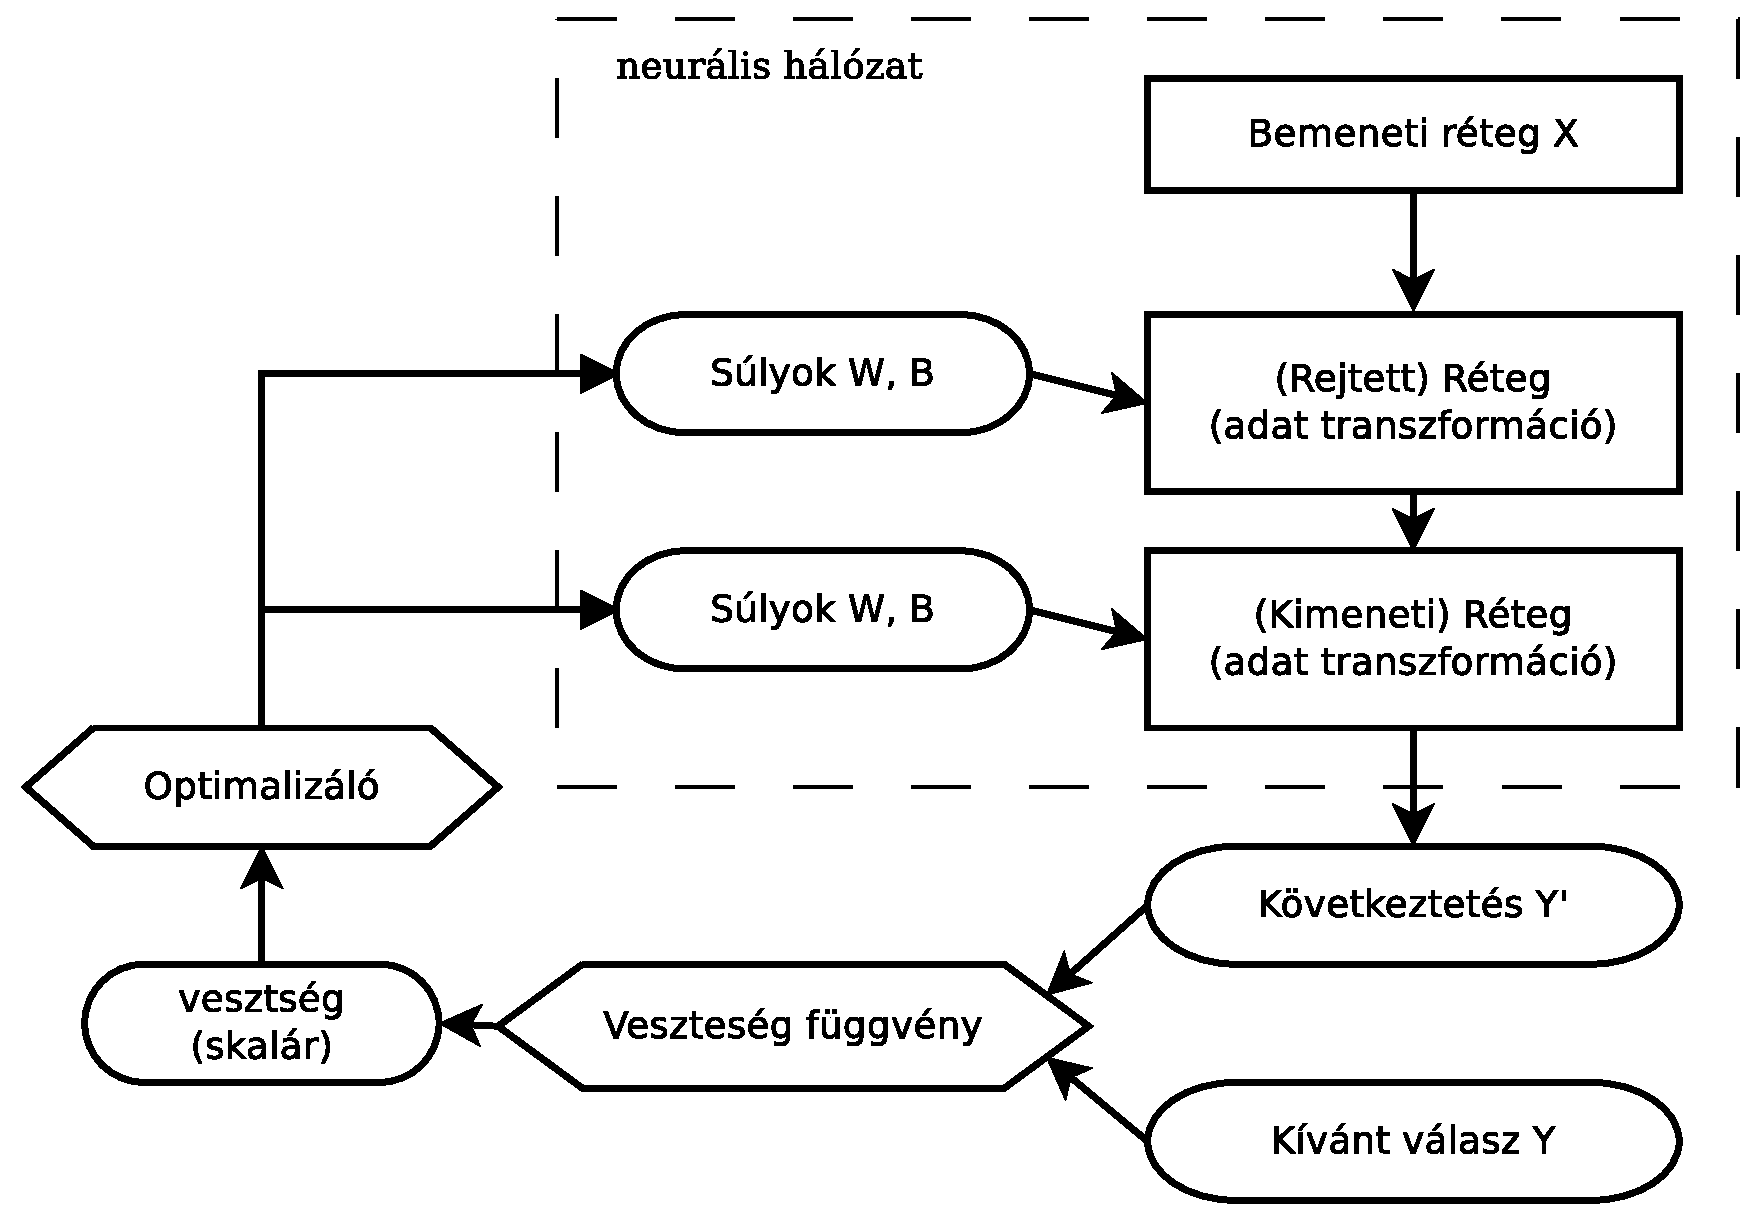
\includegraphics[width=0.7\linewidth]{fig/DNN_dia}
	\caption{A neurális hálózat tanításának folyamata}
	\label{fig:dnn}
\end{figure}

A tanítási folyamat iterációit \emph{eposzoknak} (angolul: epoch) nevezi a szakirodalom. Minden eposzban az optimalizáló hatására a kimeneti hiba csökken, a hálózat \emph{következtetése} egyre közelebb kerül az elvárthoz. 

\paragraph[SGD]{Sztochasztikus gradienscsökkentés}
A naiv megközelítést alapul véve meghatározunk egy $\eta$ tanítás sebességet (angolul: learning rate), mellyel azt befolyásoljuk, hogy egy eposzban a hálózat paramétereit mekkora mértékben változtatjuk. A tanítási sebesség az optimalizálók egy másik paramétere, tehát más eljárás esetén is alkalmazzuk valamilyen formában.
\begin{displaymath}
\vec{W_{i+1}} = \vec{W_i} - \eta\nabla C(\vec{W_i})
\end{displaymath}
Ezen paraméter változtatásánál fontolóra kell vennünk két tényezőt. Nagy tanítási sebesség gyorsabb gradiens csökkenést eredményez, ugyanakkor az elmozdulás a hibafelületen nagy kitérésekkel történik a minimumpont irányába. Túl kicsi tanítási sebességgel -- azon túl, hogy megnövekszik az eposzok szám --  ugyanakkor az optimalizálás "beragadhat" egy kedvezőtlen lokális minimum helyen.

\paragraph[RMSprop]{négzetes közép visszaterjesztése}
%RMSprop -> Root Mean Square propagation
Konstans tanulási rátát nehezen lehet jól megválasztani, ezért olyan eljárásokat dolgoztak ki, ahol ezen érték adaptálódik a tanítási folyamat során, hogy kiküszöbölje az előző bekezdésben említett nagy kitéréssel történő konvergenciát és a "beragadást". Az egyik ilyen módszer az, hogy a tanulási rátát elosztjuk az előző ciklusokban számított gradiensek nagyságának négyzetes közepével.
$$ v(w,y) = \gamma v(w,y-1) +(1-\gamma)(\nabla C(W_i))^2 $$
Ahol $\gamma$ az ún. felejtési tényező amivel szabályozhatjuk, hogy mekkora befolyása legyen az újabb gradienseknek.\\
A hálózat paramétereit a következőképpen frissítjük:
$$ W_{i+1} = W_i - \frac{\eta}{\sqrt{v(w_,y)}} \nabla C(W_i) $$
\\
Tanítás során a veszteségfüggvény sztochasztikusan konvergál a nullához és ezzel együtt a hálózat egyre pontosabban következtet a tanító készlet adataiból. A tapasztalat azonban az, hogy ez nem feltétlenül igaz más, a tanítás során nem használt adatokra, sőt elérkezhet a hálózat egy olyan állapotba, amikor a használat közben rosszabbul teljesít, mint a tanítás végén. Ilyenkor a hálózat specializálódik a tanító adathalmazra. Ezt a jelenséget, amikor a hálózat jobban következtet a tanítás során használt adathalmazon \emph{túlilleszkedésnek} nevezzük és \emph{alul-illeszkedésnek} azt, mikor a hálózat nem elég pontos, más szóval túl kevés tanítási cikluson esett még át. Hogy a hálózat a hipotézis térből a megfelelő függvények -- nem törekszünk az adatok egy tökéletes leképezésére -- valamelyikét modellezze, szükséges a tanítást felügyelni, hogy az ne illeszkedjen se túl, se alul.
A gyakorlatban ezért felügyeljük a tanítási folyamatot, és az optimalizálás minden ciklusában a hálózatnak egy külön validálásra szánt tanítókészletet adunk, és ezekre nem optimalizáljuk a hálózatot. Ezután össze tudjuk hasonlítani, hogy változik a hálózat hibája a tanító és validáló adatok mellett. Ennek tükrében abban a ciklusban ér el a hálózat a jól illesztett állapotot, amelyben a validációs veszteség érték eléri a minimumot.

\subsubsection{Regresszió optimalizálás}
%A bemeneti adatok tulajdonság szerinti normalizálása: x-átlag(x)/szórás(x) $$ s = \sqrt{\frac{1}{n-1}\sum_{i=1}^{n}(x_i - \bar{x})^2} $$
%
Osztályozási problémákon túl a mesterséges neurális hálózatok felhasználhatóak regresszióanalízisre. Ilyen feladatra tervezett hálózat kimeneti rétegének neuronjai aktivációs függvény nélküliek, tehát lineárisan képezik le a bemenetüket. Erre a kézenfekvő magyarázat, hogy a várt eredmény egy széles skálán mozoghat és bárminemű aktivációs függvény alkalmazása lekorlátozza az kimeneti adatok halmazát. Természetesen a többi réteg esetében alkalmazunk aktivációs függvényeket. Tanítás során az átlagos négyzetes hibafüggvényt --~amiről a \ref{par:mse}~bekezdésben már kitértem~-- alkalmazzuk veszteségfüggvény gyanánt. A hálózat pontosságának mérésére érdemes kiszámolni a hálózat következtetésének és az elvárt eredménynek átlagos abszolút eltérését, mint metrikát. A gyakorlatban a regressziószámítás sok változó skálán mozgó értékkel történik. A széles tartományon mozgó adatokon a hálózat nehezebben tanul, ezért a gyakorlatban érdemes a bemeneti adatokat normalizálni:
$$ s = \sqrt{\frac{1}{n-1}\sum_{i=1}^{n}(x_i - \bar{x})^2} $$
ahol $x$ a bemenő adathalmaz egy jellemzőjének egyetlen mintapontja, $n$ az egy jellemzőhöz tartozó minták száma, $\bar{x}$ pedig a minták átlaga.
Regressziószámítás a statisztikai alkalmazáson túl objektum detektálási feladatnál is felmerül: az objektumhatároló keretekhez tartozó vektorokat is többváltozós regresszióanalízissel határozhatjuk meg.
%TODO konzultálj